\section{Программный интерфейс для взаимодействия виртуальной машины с \name{Hy\-per\-led\-ger Iro\-ha}}
\subsection{Выбор интерфейса взаимодействия}
\begin{figure}[h]
 	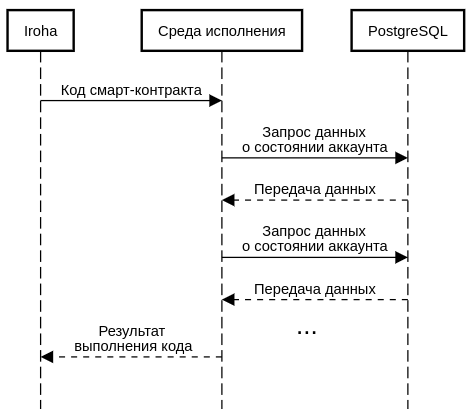
\includegraphics{interactionPog.png}
	\caption{Диаграмма последовательности взаимодействия}
	\label {interaction}
\end{figure}
На диаграмме \ref{interaction} показано взаимодействие среды исполнения с \name{Hy\-per\-led\-ger Iro\-ha} и локальной базой данных \name{PostgreSQL}, в которой хранится история транзакций, права доступа и информация о пользователях.
Среда исполнения принимает на вход код смарт-контракта и начинает его выполнение.
Для того, чтобы получать и записывать актуальное состояние переменных, среда исполнения обращается к базе данных.
Запросы выполняются по мере необходимости.
\subsection{Реализация интерфейса взаимодействия}

